\section{Connexion des caméras IP}

	L'objectif de cette mission a été d'étudier différentes caméras IP misent à ma disposition, quels sont leurs fonctionnalités, et établir un rapport qui servira à guider l'achat de nouvelles caméras.
    
    Pour cette mission, la réflexion tournera d'abord autour de l'\textbf{état de l'art}, puis sur les \textbf{difficultés rencontrées} et enfin sur des \textbf{améliorations possibles} à l'étude de connexion des caméras IP.

  \subsection{État de l'art}
  
  L’état de l'art se décompose ici en l'étude des \textbf{caméras IP} et des \textbf{solutions existantes} pour la connexion de ces caméras
 	 \subsubsection{Les caméras IP}
        Une \textit{caméra IP}, est une \textbf{caméra numérique} généralement utilisée pour la \textbf{surveillance}. Contrairement à des caméras dites CCTV (\textit{Closed-circuit television}), la caméra IP peut envoyer et recevoir des données via un \textbf{réseau informatique et internet}. Bien que la plupart des caméras pouvant faire cela sont des webcams, le terme \textit{caméra IP} est généralement utilisée 
dans le cadre de la surveillance qui peut être directement accédé par une connexion réseau.
        
        Une caméra IP peut être câblée avec du \textit{RJ45} vers un \textit{routeur} ou «~box ADSL~», ce qui lui permet à la fois d'être alimentée et les images visionnées sur le réseau, ou alors par Wi-Fi (une alimentation en courant électrique devient alors nécessaire). \textbf{Contrairement aux Webcams}, la compatibilité avec les logiciels de visioconférence n'est pas toujours garantie.
        
 	 \subsubsection{Solutions existantes}
     
     La connexion aux caméras IP n'est pas un monde vierge de toute fondation, on y trouve des \textbf{interfaces}, des \textbf{flux \textit{RSTP}}, et une \textbf{norme \textit{Onvif}}
     
		\subTrois{Les interfaces constructeurs}
        Les caméras IP sont en règle générale accompagnées dans leur partie logicielle d'une interface utilisateur. Ces interfaces permettent de configurer les caméras et éventuellement d'accéder au flux vidéo. L'approche de conception de ces interfaces varie grandement en fonction du public visé et de l'utilisation préconisée.

Voici quelques exemples d'interface rencontrée au cours du stage :
\begin{itemize}
\item         \textbf{D-Link}, une interface complète, localisée en français, conçue pour être facilement configurable par des professionnels et des amateurs, bien qu'elle nécessite la connaissance de son adresse IP pour y accéder.
\item         \textbf{XIAOMI, Xiao Fang (Fang Hacks)}, XIAOMI n'étant pas encore implanté en France quand il a fallu essayer ce modèle (avant le 22 mai 2018~\cite{Xiaomi}), son service de Cloud n'était \textit{a fortiori} pas non plus accessible sur le territoire français. Il a fallu installer nouveau système d'exploitation sur la caméra, le \textit{«~Fang Hacks~»}~\cite{FangHacks}. Cette interface est très rudimentaire et ne contient qu'une interface destinée à gérer la connexion. Elle s'adresse surtout à un  public de technophiles ayant envie d'utiliser cette caméra premier prix.
\item         \textbf{VR CAM}, marque d'origine chinoise, cible un très grand public et permet de connecter et d'utiliser leurs caméras via leur application mobile~\cite{VRCam}. Une utilisation via une autre médium n'est pas prévue par le constructeur. L'interface de l'application a visiblement été localisée en utilisant un traducteur automatique à partir du chinois.
\end{itemize}


\begin{minipage}{0.3265\textwidth}
\begin{figure}[H]
	\centering
	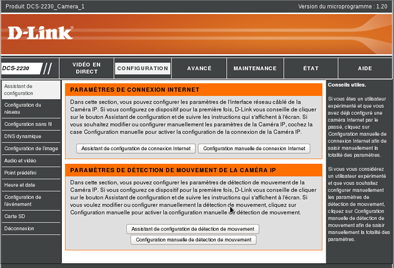
\includegraphics[width=4.5cm]{img/d-link_web.png}
    \caption{\\D-Link}
\end{figure}
\end{minipage}
\begin{minipage}{0.3265\textwidth}
\begin{figure}[H]
	\centering
	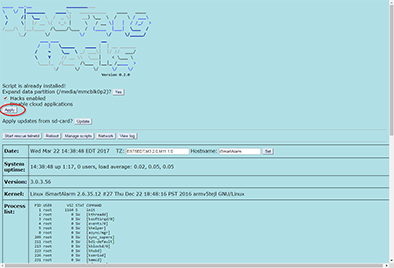
\includegraphics[width=4.5cm]{img/fanghacks.png}
    \caption{\\Fang Hacks}
\end{figure}
\end{minipage}
\begin{minipage}{0.3265\textwidth}
\begin{figure}[H]
	\centering
	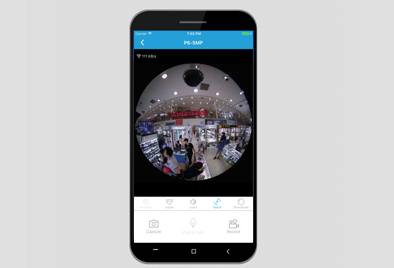
\includegraphics[width=4.5cm]{img/vrcam_mob.png}
    \caption{\\VRCAM}
\end{figure}
\end{minipage}
        
		\subTrois{Le RTSP}
\textit{RTSP} ou \textit{Real Time Streaming Protocol} (protocole de streaming temps-réel) est un protocole de communication de niveau applicatif(niveau 7 du modèle \textit{OSI}) destiné aux systèmes de streaming média. Il permet de \textbf{contrôler un serveur de média} à distance, offrant des fonctionnalités typiques d'un lecteur vidéo telles que «~lecture~» et «~pause~», et permettant un accès en fonction de la position temporelle.~\cite{RTSPwiki}

La \textbf{transmission des données} de streaming elle-même n'est pas la tâche du protocole \textit{RTSP}. La plupart des servers \textit{RTSP} utilise le \textit{RTP} (\textit{Real-time Transport Protocol}) en conjonction avec \textit{RTCP} (\textit{with Real-time Control Protocol}) pour la distribution du stream média.~\cite{RTSP}

Le \textit{RTSP} permet le \textbf{multicast} pour la diffusion simultanée à plusieurs clients. Une variété de formats vidéos et audio sont supportés tel que .\textit{264}, \textit{MPEG4}, \textit{MJPEG}, \textit{AAC}, \textit{WMV} etc.

Son utilisation peut se faire avec le logiciel de lecture vidéo \textit{VLC}, ou par un programme qui utilise la librairie \textbf{OpenCV} par exemple.

		\subTrois{La norme \textit{Onvif}}
        
          \begin{minipage}{0.2\textwidth}
  \centering
  
\includegraphics[width=4cm]{img/logoonvif.png}
\end{minipage}
\hfill%
\begin{minipage}{0.7\textwidth}
Le protocole \textit{ONVIF}~\cite{Onvif} est l'acronyme du \textbf{O}pen \textbf{N}etwork \textbf{V}ideo \textbf{I}nterface \textbf{F}orum. Le principe remonte au début des années 2010, où les grandes marques du domaine telles que \textit{Sony} ou \textit{Bosch} ont proposé de mettre en place un forum industriel qui vise à développer une \textbf{norme mondiale d'inter-opérabilité} des produits de sécurité IP. 
  \end{minipage}\par
  
  \textit{ONVIF} travaille aussi avec des groupes de standardisation tel qu'\textit{IEC} (\textit{International Electrotechnical Commission}), \textit{CENELEC} et \textit{ISO} pour leur faire adopter les spécifications ONVIF. Ces spécifications sont des services web, utilisent des standards ouverts dont \textit{XML}, \textit{SOAP} et \textit{WSDL} pour définir la communication entre deux appareils électroniques dans un réseau IP.

Ceci permet aux produits de vidéo-surveillance IP \textbf{de pouvoir échanger des informations} entre eux, même s'ils proviennent \textbf{de différent fabricants}. Cependant il appartient à ces fabricants d'implémenter ce standard dans leurs produits. Toutes les caméras Onvif n'auront pas la même liste exhaustive de contrôles, ni la même qualité d'implémentation.

La connexion via le protocole Onvif peut se faire en passant par le logiciel open source \textit{ONVIF Device Manager}~\cite{Onvifdm}. Pour la connexion, il suffit de renseigner l’adresse \textbf{[IP]:[Port Onvif]} de la caméra concernée en utilisant l'interface du logiciel.

\begin{figure}[H]
	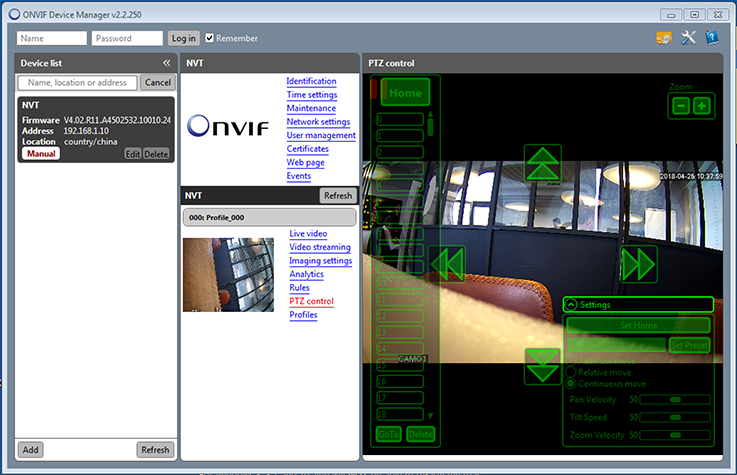
\includegraphics[width=0.7\textwidth]{img/onvifecran.png}
    \centering
    \caption{Interface d'\textit{ONVIF Device Manager}}
\end{figure}

Durant cette mission, des difficultés ont été rencontrées.

	\subsection{Difficultés rencontrées}

Les caméras qui m'ont été demandées d'étudier ne venaient pas toujours avec toutes les clefs. Cela s'illustre par :
\begin{enumerate}
\itemsep -0.5em 
\item la documentation parfois lacunaire,
\item des soucis pour les connecter au réseau,
\item une compatibilité logicielle,
\item des formats de flux vidéo.
\end{enumerate}


		\subsubsection{La documentation}
Lors de ma mission, certaines caméras à connecter n'avaient pas forcément une documentation très fournie.

Par exemple une caméra (\textit{Escam Q1039}) avait comme  documentation officielle une vidéo sur youtube en russe.

\begin{figure}[H]
	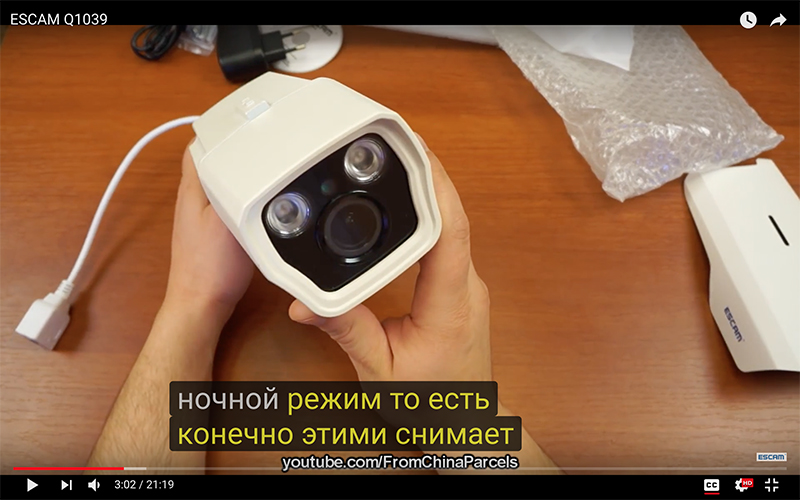
\includegraphics[width=0.8\textwidth]{img/escam_russe.jpg}
    \centering
    \caption{vidéo explicative en russe\\publiée sur la chaîne Youtube d’EScam~\cite{EscamVid}}
    \end{figure}
    Le manque de documentation peut s'avérer problématique. En effet, chaque fabricant dans l'installation de la partie logiciel de la caméra attribut notamment des adresses pour accéder aux flux vidéos pour \textbf{RTSP} ou \textbf{Onvif} par exemple.
    
    Toutefois, il reste possible de parfois retrouver certaines de ces informations. Par exemple le site \textit{ipsyConnect} met à disposition une liste de caméra avec des adresses pour se connecter en \textit{RTSP}.~\cite{ispy}
\begin{figure}[H]
    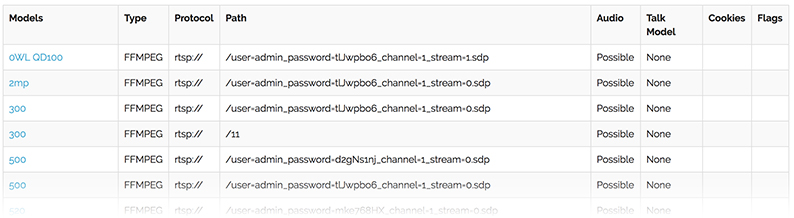
\includegraphics{img/liste_ispy.jpg}
    \centering
    \caption{extrait de la liste de caméra EScam sur ISpyConnect}
\end{figure}

		\subsubsection{La connexion au réseau}
    Pour configurer une caméra IP une connexion au routeur internet est nécessaire.
        
	L'installation des locaux de la «~\textit{Forge}~» est faite de telle façon à ce qu'internet soit accessible par wi-fi uniquement. L'accès au routeur n'est pas possible. La connexion a donc dû se faire sans passer par le réseau internet. Pour établir une connexion, la connexion s'est établie en pair à pair avec deux nœuds en branchant directement un câble \textit{RJ45} à l'ordinateur et à la caméra IP.
    
    Cette configuration réseaux particulière a permis d'explorer les fonctionnalités des caméras, mais sans avoir accès un internet ce qui a pu poser problème lors de la recherche d'informations au cours de l'utilisation.
    
		\subsubsection{La compatibilité logicielle}
	Durant le stage j'utilise mon ordinateur personnel. Un Macbook Pro avec \textbf{MacOS}. Cependant certains logiciels ne sont pas compatible avec ce système d'exploitation. Un appareil a même son interface web qui utilise \textbf{ActiveX}. ActiveX n'est compatible qu'avec \textbf{Internet Explorer} qui n'est pas compatible avec MacOs. 
    
    Pour contourner ce problème j'ai dû installer une \textbf{Machine Virtuelle Windows} pour lancer Internet Explorer et y utiliser Active X.
\begin{figure}[H]
    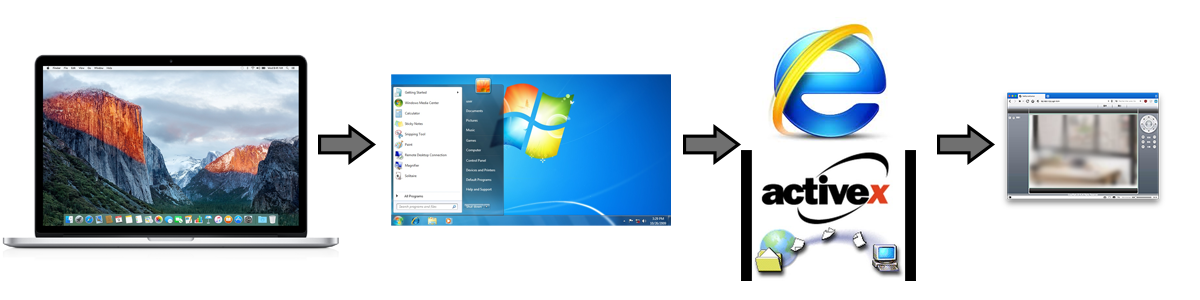
\includegraphics[width=0.8\textwidth]{img/Aesthetic_graph.png}
    \centering
    \caption{Environnement de travail ad hoc}
\end{figure}

    \subsubsection{Le format de flux vidéo}
    Chaque fabricant ayant le droit de faire comme bon lui semble, certaines caméras peuvent avoir des formats de flux vidéos qui ne sont pas exploitables. En effet, il est arrivé qu'une caméra ne retourne pas un flux vidéo, mais une image au format \textit{.jpeg} en se connectant avec l'adresse \textbf{RTSP}. Cette méthode a réputation d'avoir des images de meilleures qualité au prix d'une vidéo plus saccadée. Avec une vidéo mois fluide, l'étude du déplacement d'un objet est plus compliquée.

Il a été décidé d'écarter les caméras qui renvoient un flux d'image qui n'est pas au format vidéo. 

Des \textbf{améliorations sont possibles}. 

\subsection{Améliorations possibles}

  L'étude des caméras c'est fait à partir d'un nombre réduit de caméras (quatre). Pousser l'étude consisterai à \textbf{augmenter le nombre de caméras}. Ainsi de nouveaux problèmes vont se dévoiler et alors de nouveaux critères vont émerger pour \textbf{affiner le guide pour l'achat de caméras}.

  Un autre aspect serait de pouvoir \textbf{connecter les caméras à un router et y accéder à distance}. En raison des limitations techniques cet aspect à été mis entre parenthèse, mais il reste néanmoins un aspect fondamental des caméras IP.

% ------------------------------------------------
% /\/\/\/\/\/\/\/\/\/\/\/\/\/\/\/\/\/\/\/\/\/\/\/\
% ------------------------------------------------
\cleardoublepage
\section{Établissement d'un protocole de test de caméras}
La deuxième partie de ma mission d'étude de caméra est d'effectuer un travail de veille. Il sert à établir un protocole de test de ces caméras. Ces tests ont pour vocation d'estimer la qualité des enregistrements vidéos et d'en reconnaître les plus adaptés au besoin de la \textit{Computer Vision}.  

La présentation de cette mission commence par un \textbf{état de l'art}, suivie d'une de ma \textbf{contribution} qui sera ensuite \textbf{évaluer} et des \textbf{perspectives} possibles.

  \subsection{État de l'art}
    Les tests de qualité des caméras est essentiellement basée sur l'évaluation de la netteté de l'image. Les sociétés qui effectuent les tests de caméras ont leurs propres méthodologies, mais ont tendance à s'inspirer de la \textbf{norme ISO-12233}~\cite{ISO12233}. Cette norme présente notamment un panneau qui sert à évaluer la netteté de l'image. Cette norme est mise à jour environ tout les quatre ans. La dernière version en date est celle de 2017.

  \begin{minipage}{0.45\textwidth}
  \begin{figure}[H]
      \centering
      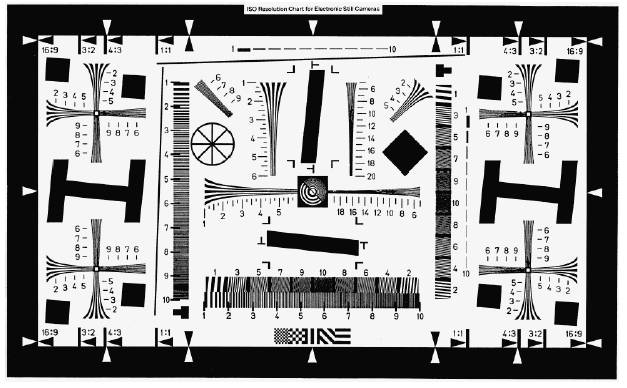
\includegraphics[width=6cm]{img/ISO12233-2000.jpg}
      \caption{ISO12233-2000}
  \end{figure}
  \end{minipage}
  \begin{minipage}{0.5\textwidth}
  \begin{figure}[H]
      \centering
      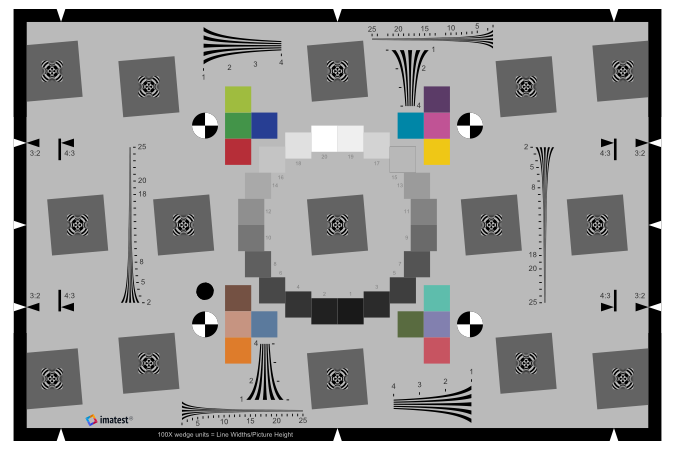
\includegraphics[width=6cm]{img/ISO12233-2017.png}
      \caption{ISO12233-2017}
  \end{figure}
  \end{minipage}

    La netteté est analysée à partir de zébrures de plus en plus resserrées, plus l'image sera nette, plus chacune de ses rayures seront distinctes. L'analyse se fait avec des algorithmes dit de \textbf{MTF} (pour \textbf{M}odulation \textbf{T}ransfer \textbf{F}unction)~\cite{MTF}. Plusieurs programmes payants permettent ces analyses (\textit{IMATEST}, \textit{QuickMTF}), il est également possible d'utiliser un script python avec des librairies gratuites. Les résultats obtenus vont toutefois varier en fonction de l'implémentation de l'algorithme.

    \begin{figure}[H]
      \centering
      
\includegraphics[width=0.8\textwidth]{img/mtf.png}
      \caption{Effet de perte de netteté sur les zébrures}
  \end{figure}

  Les panneaux de la norme \textbf{ISO-12233} disposent des rayures de façon à prendre en compte les courbures de la lentille de l'appareil. L'image ayant tendance à être plus nette au centre que sur les bords.
  
  Pour avoir une meilleure luminosité de la façon la plus consistante possible, les images sont prises en intérieur, avec des lumières neutres et en utilisant des panneaux servant filtrer la lumière pour la rendre plus diffuse et éviter les reflets.
  
  La capacité d'une caméra à produire une image nette varie en fonction de plusieurs facteurs comme la \textbf{luminosité}, la \textbf{distance focale} ou le \textbf{mouvement}. 
  
  \subsection{Contributions}
  La finalité de cette mission a été de \textbf{présenter un document} qui compile les conclusions du \textbf{travail de veille} pour les caméras. Ce document a pris la forme d'une présentation \textit{Microsoft Power Point}.
  
  Une solution naïve pour les tests de caméra dans un environnement \textbf{contrôlable et prédicable} est de filmer un écran qui diffuse une vidéo. Cette solution permet en théorie de contrôler simplement toutes les variables comme la luminosité, les éléments de l'image, le mouvement. Une solution idéale en théorie, en pratique elle présente plusieurs \textbf{inconvénients}.
  
  Filmer un écran qui diffuse une vidéo ne revient pas au même que de filmer directement la vidéo. L'écran est plat, projette de la lumière et en reflète. Ceci a pour effet de dégrader fortement la qualité de l'image. En conséquence l'image que filme la caméra n'est plus de qualité suffisante pour tester la qualité de l'image en situation réelle.
  
	\begin{figure}[H]
      \centering
      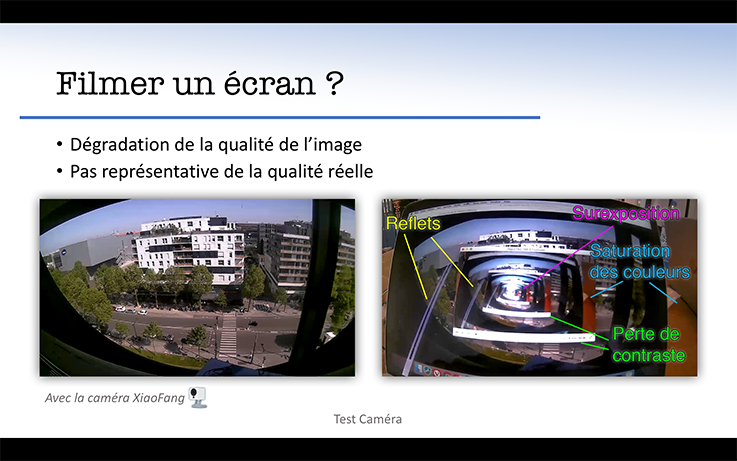
\includegraphics[width=12cm]{img/CamTestEcran.png}
      \caption{Écarter explicitement cette solution\\et pourquoi}
	\end{figure}
  
  La solution retenue utilise donc un support \textbf{analogique} pour une meilleure fidélité d'image.
  
  L'installation voulue serait une installation qui correspond à l'état de l'art (lumière neutre, panneau diffuseur de lumière, trépied pour la caméra) et sans un logiciel particulier pour évaluer la netteté. La luminosité ayant un effet important sur la qualité d'image, l'utilisation d'un \textbf{photomètre}, appareil servant à mesurer les niveaux de luminosité, est recommandé pour s'assurer des bonnes conditions de tests.
  
  Les tests principaux se font en utilisant un \textbf{panneau ISO-12233} compatible.
  
\begin{minipage}{0.4\textwidth}
  \begin{figure}[H]
    \centering
    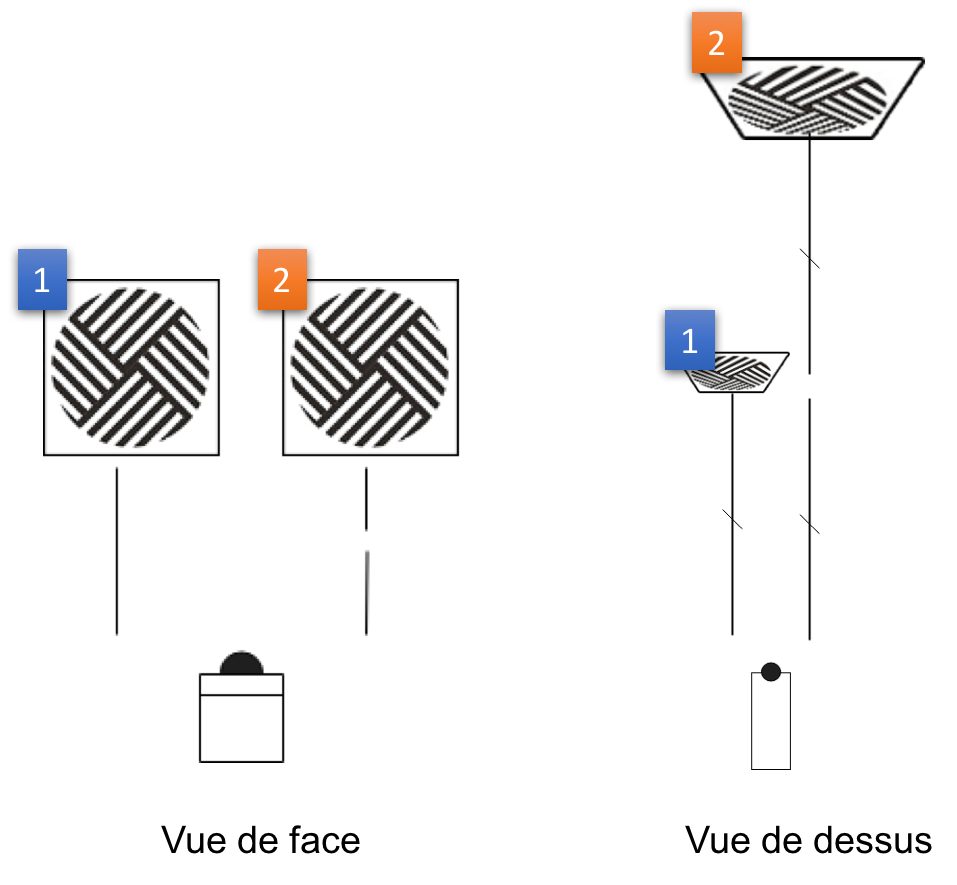
\includegraphics[width=\textwidth]{img/test_focal.png}
    \caption{schéma pour l'installation des tests de focal}
  \end{figure}
\end{minipage}
\hfill%
\begin{minipage}[adjusting]{0.52\textwidth}
  Les vidéos devant tenir compte de la \textbf{profondeur de champ}, il est intéressant de chercher à s'assurer que les caméras retenues puissent offrir une bonne qualité d'image à différent niveau de profondeur.
L'idée pour ce test est de prendre deux panneaux, de tailles différentes placés à une distance calculée telle que les deux panneaux apparaissent de même taille. On analyse la netteté de l'image avec les deux panneaux. \textbf{Si la caméra est capable de bien gérer bien les profondeurs d'image, les deux panneaux seront nets}. Sinon, un panneau sera plus flou que l'autre. 
\end{minipage}\par

Pour l'analyse de la \textbf{qualité d'image lors du mouvement}, un autocollant posé sur un démonstrateur capable de le déplacer selon un trajet défini. On analyse la netteté de l'image lors du déplacement sur plusieurs directions.


\begin{minipage}{0.2\textwidth}
\begin{figure}[H]
    
\includegraphics[width=0.5\textwidth]{img/grille_couleur.png}
    \centering
    \caption{exemple de grille de couleur}
\end{figure}
\end{minipage}
\hfill%
\begin{minipage}[adjusting]{0.7\textwidth}
Un autre critère qui n'est pas lié à la netteté de l'image est la \textbf{fidélité des couleurs}. Certains algorithmes de Computer Vision passent par une sélection de couleur. Pour tester la fidélité, on capture l'image d'un panneau avec une grille de couleurs avec des valeurs cibles connues. 
\end{minipage}\par

\subsection{Évaluation et perspectives}

La démarche de protocole de test ne \textbf{s'est jamais concrétisée}. Les moyens à mettre en place n'étaient pas justifiés par le besoin estimé de réaliser ces tests. Sans réaliser ces tests il est \textbf{difficile d'estimer la pertinence} de certain d'entre eux.

Par exemple tester \textbf{à différent niveau de luminosité} lors de chaque test. Avec trois niveaux de luminosité (jour, pluie et nuit), le nombre de tests se multiplie donc par trois. Le temps de réaliser ces tests augmente d'autant plus qu'il faut compter le temps de changer le niveau et s'assurer que la luminosité est correcte en la mesurant à chaque fois. On peut se demander si la différence que provoque les écarts de luminosité diffère significativement entre un test de focale, de mouvement ou juste pour un panneau simple.

Le démonstrateur qui déplace la zébrure pour le test \textbf{en mouvement} n'est pas très rapide. J'avais réfléchi  à un système avec différents cylindres superposés avec des vitesses de rotations différentes. Le souci c'est qu'il aurait fallu une imprimante 3D pour produire les pièces (cylindres, rouages...), un logiciel de modélisation 3D pour créer les fichiers à imprimer, se former en électronique et en mécanique, acheter du matériel électronique (\textit{arduino}, \textit{breadboard}...). Dans la mesure où avec le démonstrateur les tests n'étaient pas une priorité, mettre en place ce test aurait demandé un effort bien trop important pour cette mission.
\begin{figure}[H]
    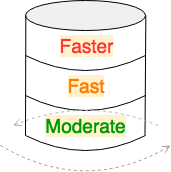
\includegraphics[width=0.15\textwidth]{img/vit_cyl.png}
    \centering
    \caption{schéma rudimentaire\\du projet de test de netteté en mouvement}
    \end{figure}
  Ce qui a été accompli a servi à constituer un document avec des observations et des recommandations qui seront peut-être réutilisés, quand le besoin de tester des caméras se présentera pour l'équipe.
  
  La poursuite du développement de ces protocoles de tests ne semble pas être une priorité pour le moment.